\documentclass[a4paper]{article}
\usepackage[french]{babel}
\usepackage[T1]{fontenc}
\usepackage[utf8x]{inputenc}
\usepackage{a4wide,textcomp,graphicx,keystroke,amssymb,amsmath,listings,pifont,color,fourier-orns}
\title{\textbf{Spécification d'un outil de visualisation de pavages}}
\author{ JERMANN.C MARGUERITE.A}
\date{\today}


%%%%%%%%%%%%%%%%%%%%%%%%%%%%%%%%%%%%%%%%%%%%%%%%%%%%%%%%%%%%%%%%%%%%%%%%%%%%%%%%%%%
%%%%%%%%%%%%%%%%%%%%%%%%%%%%%%%%%%%%%%%%%%%%%%%%%%%%%%%%%%%%%%%%%%%%%%%%%%%%%%%%%%%
%%%%%%%%%%%%%%%%%%%%%%%%%%%%%%%%%%%%%%%%%%%%%%%%%%%%%%%%%%%%%%%%%%%%%%%%%%%%%%%%%%%
\begin{document}
\maketitle{}
\renewcommand\labelitemi{\textbullet}

\paragraph{Introduction :} L'objectif est de définir un outil de visualisation d'une projection en une, deux ou trois dimensions d'un pavage à N dimensions typiquement produit par un outil de résolution par intervalles de problèmes numériques (tel que Realpaver). Cet outil permettra de visualiser entièrement ou partiellement le pavage et d'ajuster les propriétés graphiques de la visualisation, puis d'exporter le résultat. Une indépendance vis à vis du logiciel fournissant les données est requise. Le traducteur pour passer du format de sortie du logiciel source au langage d'entrée dédié à l'outil de visualisation n'entre pas dans la conception.
\paragraph{Mise en garde}
Il existe des différences entres les les images et le texte. Ces différences seront signaler par le symbole $\triangle$ .Dans tous les cas se référer en priorité au texte
%%%%%%%%%%%%%%%%%%%%%%%%%%%%%%%%%%%%%%%%%%%%%%%%%%%%%%%%%%%%%%%%%%%%%%%%%%%%%%%%%%%
\section{Format d'entrée}

%----------------------------------------------------------------------------------
\subsection{Généralités}
\begin{itemize}
\item Une entrée = un pavage ; l'entrée peut-être dynamique si le pavage est en cours de production.
\item Format : texte au codage UTF-8
\item L'entrée comporte une partie entête et une partie corps ; l'entête se place obligatoirement avant le corps.
\item Les identifiants des données sont soit des chaînes de caractères (IDStr) restreintes aux lettres, aux chiffres et à l'underscore et commençant obligatoirement par une lettre (e.g., variables, caractéristiques, ...), soit des entiers positifs (IDInt) (e.g., boites, points de référence, ...). Dans tous les cas, l'identifiant est unique.
\item Les types des données manipulées sont : Number, Interval et String.
\item Les valeurs de type String sont des chaines de caractères comprises entre guillemets (") et pouvant contenir tout caractère à l'exception des guillemets.
\item Les données de type Number sont représentées par des flottants (cf. norme IEEE 754).
\item Les données de type Interval sont représentées par deux données de type Number.
\end{itemize}

%----------------------------------------------------------------------------------
\subsection{Entête}\label{sec:entree:entete}
Les éléments marqués d'un astérisque peuvent être omis.
\begin{itemize}
\item Nombre de boîtes (entier positif, type Number). Lorsque l'entrée est dynamique, cette valeur est inconnue (remplacée par un tag ou une valeur spécifique, e.g., 0).
\item Liste des identifiants (IDStr) des variables (ordre important).
\item (*) Liste des identifiants (IDStr) et types (Number, Interval ou String) des caractéristiques (e.g., temps de calcul, précision, certification) associées aux boîtes (ordre important).
\item (*) Liste des points de références, chacun composé de :
  \begin{itemize}
  \item identifiant (IDInt)
  \item label (court texte, type String)
  \item commentaire (texte plus long, optionnel, type String)
  \item coordonnées (autant que de variables, type Number)
  \item caractéristiques d'affichage :
    \begin{itemize}
    \item[.] Couleur : code RVB (type String)
    \item[.] Taille des points (en pixels, type Number)
    \item[.] Police du label (type String) et son style (gras, italique, gras-italique)
    \end{itemize}
  \end{itemize}
\item (*) Liste des filtres. Un filtre détermine un ensemble de boites à afficher. Les filtres sont considérés en disjonction : toute boite satisfaisant au moins un filtre est affichée. Chaque filtre se définit au moyen d'une règle, semblable à celle composant un affichage conditionnel. Chaque filtre est composé de :
  \begin{itemize}
  \item identifiant (IDInt)
  \item label (court texte, type String)
  \item règle : liste de conditions (considérées en conjonction) ; chaque condition est composée de :
    \begin{itemize}
    \item[.] un élément testé : l'identifiant (IDInt) d'une boite, la valeur (Interval) d'une variable (IDStr), la valeur (selon son type) d'une caractéristique (IDStr), ou une formule (Interval) combinant des variables au moyen d'opérations mathématiques.
    \item[.] une relation, selon le type d'élément testé\\
      IDInt boite : $=$, $\neq$, $<$, $\leq$, $>$, $\geq$\\
      Interval : $\ni$, $\not\ni$, $<_{inf|sup}$, $\leq_{inf|sup}$, $>_{inf|sup}$, $\geq_{inf|sup}$\\
      String : $=$, $\neq$, $\ni$, $\not\ni$
    \item[.] une valeur comparative, selon le type d'élément testé\\
      IDInt boite : un entier positif\\
      Interval : une valeur de type Number\\
      String : une valeur de type String
    \end{itemize}
  \end{itemize}
\item (*) Liste des affichages conditionnels. Un affichage conditionnel définit comment doivent apparaître les boites vérifiant certaines conditions. Les affichages conditionnels sont considérés en disjonction et dans l'ordre de leur définition (toute boite s'affiche selon les modalités du premier affichage conditionnel dont elle remplit les conditions). Chaque affichage conditionnel est composé de :
  \begin{itemize}
  \item identifiant (IDInt)
  \item label (court texte, type String)
  \item règle (cf. Filtres)
  \item style, définissant les modalités d'affichage des boites validant la règle, c'est-à-dire sa couleur (avec transparence, code RVBA, type String)
  \end{itemize}
\item (*) Définition du point de vue :
  \begin{itemize}
  \item Liste des 1, 2 ou 3 variables visualisées
  \item Les coordonnées de la caméra définissant le mapping 1/2/3D$\to$2D (cf. http://en.wikipedia.org /wiki/3D\_projection) ; sera défini précisément une fois la technologie utilisée pour la visualisation déterminée.
  \end{itemize}
\end{itemize}

%----------------------------------------------------------------------------------
\subsection{Corps}
Liste de boîtes du pavage, chacune comprenant :
\begin{itemize}
\item identifiant (IDInt)
\item Liste des coordonnées (type Interval) de chaque variable dans la boite, dans l'ordre dans lequel les variables sont listées dans l'entête.
\item Liste des caractéristiques, dans lordre et selon les types définis en entête
\end{itemize}

%%%%%%%%%%%%%%%%%%%%%%%%%%%%%%%%%%%%%%%%%%%%%%%%%%%%%%%%%%%%%%%%%%%%%%%%%%%%%%%%%%%
\section{Présentation de l'IHM générale}
\paragraph{Note sur les informations de spécifications}
Les spécifications seront dans cette partie décrite textuellement et illustrées. Les illustrations peuvent être incomplète et il est necessaire de s'appuyer sur le texte pour les spécifications exactes. Dans la mesure du possible les éléments manquant dans les illustrations seront annotés par $\triangle$ 
On trouvera 5 composantes dans la fenêtre de l'outil :
\begin{itemize}
\item Une barre de menu en haut.
\item Une barre d'outils située sous la barre de menu.
\item Une partie centrale de visualisation.
\item Un panneau latéral-droit d'édition et d'information.
\item Une barre d'état en bas.
\end{itemize}

\paragraph{Remarque :} Lors du redimensionnement de la fenêtre de l'application, seule la partie centrale de visualisation sera redimensionnée ; le panneau latéral aura une largeur fixe et une hauteur minimale qui définira aussi la hauteur minimale de la fenêtre d'application. Ni la partie centrale ni le panneau latéral ne seront dotés de barres de défilement.

\begin{figure}[h]
  \center
  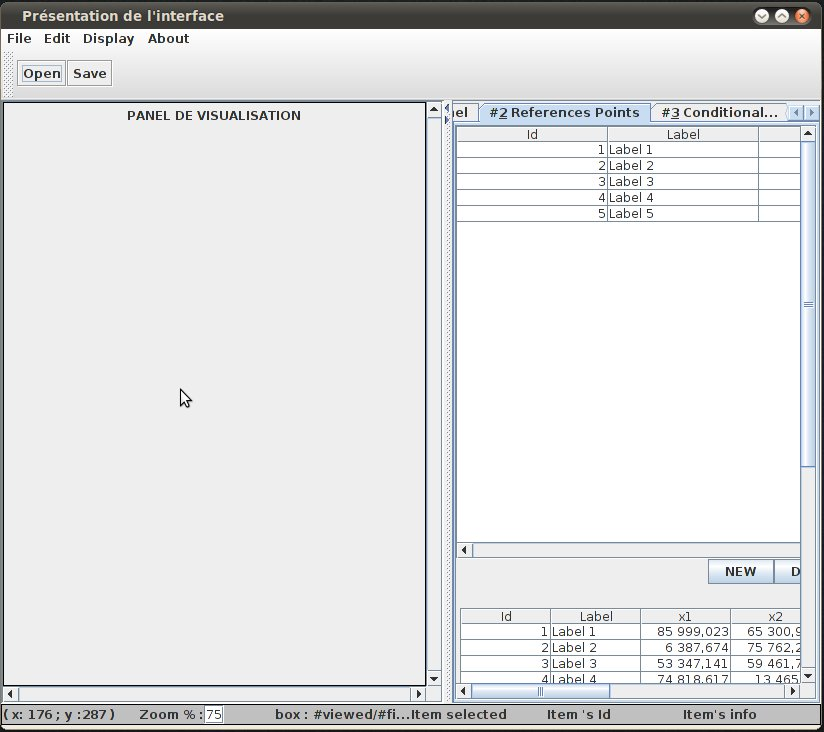
\includegraphics[scale=0.40]{spec-images/ihm_generale.jpeg}
  \caption{IHM générale}
\end{figure}

%----------------------------------------------------------------------------------
\subsection{Barre de menu}
Elle est composée des sous-menus :

\begin{tabular}{cc}
\begin{minipage}{0.5\linewidth}
\begin{itemize}
\item File :
  \begin{itemize}
  \item Open
  \item Save
  \item Export as image
  \item Quit
  \end{itemize}
\item Edit :
  \begin{itemize}
  \item Preferences
  \item Create a Ref. Point
  \item Select
    \begin{itemize}
    \item[.] All
    \item[.] by Id
    \item[.] by Coord.
    \end{itemize}
  \end{itemize}
\end{itemize}
\end{minipage}
&
\begin{minipage}{0.5\linewidth}
\begin{itemize}
\item Display
  \begin{itemize}
  \item Choose variables
  \item Zoom
    \begin{itemize}
    \item[.] All
    \item[.] In
    \item[.] Out
    \end{itemize}
  \end{itemize}
\item Help :$\triangle$
  \begin{itemize}
  \item Help 
  \item About
  \end{itemize}
\end{itemize}
\end{minipage}
\end{tabular}

%----------------------------------------------------------------------------------
\subsection{Barre d'outil} 
Elle est composée d'icônes (raccourcis) d'items de la barre de menu décrite précédemment. Son contenu est paramétrable par l'utilisateur. Les éléments suivants y sont toujours présents :
\begin{itemize}
\item les ID des variables visualisées (3 combobox éditables comprenant chacun la liste de toutes les variables).$\triangle$
\item Le zoom homogène, i.e., égal sur toutes les dimensions (1 champ texte éditable et 2 boutons "+" et "-").$\triangle$
\end{itemize}

%----------------------------------------------------------------------------------
\subsection{Menu contextuel(à compléter)}
Menu s'ouvrant lors d'un clic du bouton droit de la souris dans la zone de visualisation. Il contient les éléments suivants :
\begin{itemize}
\item Create a Ref. Pt
\item Zoom All
\item Zoom In
\end{itemize}

%----------------------------------------------------------------------------------
\subsection{Panneau de visualisation}
C'est ici que l'on observera la représentation graphique 1, 2 ou 3D du pavage. Il sera interactif avec la souris et le clavier (cf partie \ref{sec:visualisation}).

%----------------------------------------------------------------------------------
\subsection{Panneau latéral}
Il est composé de 4 onglets :
\begin{itemize}
\item Box (cf partie \ref{sec:onglet:box})
\item Reference Points (cf partie \ref{sec:onglet:rpt})
\item Filters (cf partie \ref{sec:onglet:flt})
\item Conditional Style (cf partie \ref{sec:onglet:aff})
\end{itemize}

%----------------------------------------------------------------------------------
\subsection{Barre d'état}
Elle est contient divers information générales sur les données de l'application :
\begin{itemize}
\item L'ID de l'item survolé.
\item Les coordonnées de la souris dans le panneau de visualisation.
\item Le nombre de boites vues/filtrées/total.
\end{itemize}

%%%%%%%%%%%%%%%%%%%%%%%%%%%%%%%%%%%%%%%%%%%%%%%%%%%%%%%%%%%%%%%%%%%%%%%%%%%%%%%%%%%
\section{Panneau latéral}

%----------------------------------------------------------------------------------
\subsection{Onglet Box}\label{sec:onglet:box}

\begin{figure}[h]
  \center
  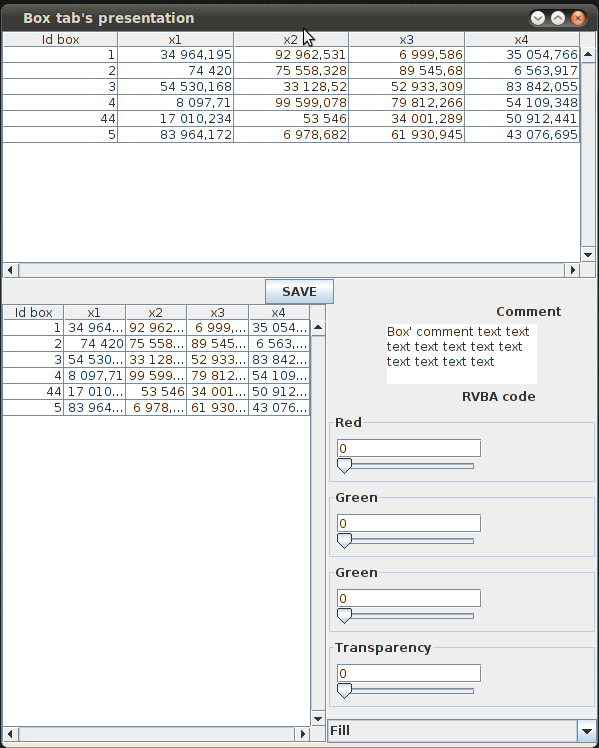
\includegraphics[scale=0.50]{spec-images/Onglet_Box.png}
  \caption{Onglet de visualisation des caractéristiques des boîtes }
\end{figure}
Essentiellement dédié à la lectures d'informations complémentaires de la visualisation. Il contient 4 parties :
\begin{itemize}
\item Dans la partie supérieure, une liste des boites donnant leurs ID, les valeurs (intervalles) des variables visualisées (1, 2 ou 3), la liste des ID des filtres dont la règle est validée par la boite $\triangle$, l'ID de l'affichage conditionnel qui s'applique à la boite $\triangle$. Cette liste pourra ne comporter que les boites actuellement visualisées, que celles satisfaisant au moins un filtre, ou l'intégralité des boites du pavage en entrée (choix au moyen d'un radio-bouton$\triangle$). Elle pourra être réordonnée, de façon croissante ou décroissante, selon les ID ou les valeurs des variables visualisées (selon la borne inférieure de l'intervalle). Si la liste excède la taille de la zone dédiée, une barre de défilement verticale apparaît. La sélection, par clic gauche de la souris, d'une boite de la liste la met également en surbrillance dans la fenêtre de visualisation. Réciproquement, la sélection d'une boite dans la zone de visualisation sélectionne automatiquement celle-ci dans la liste.
\item Dans la partie inférieure gauche, les informations (non éditables) détaillées de la boîte sélectionnée dans la zone supérieure : la liste des valeurs de toutes les variables, munie au besoin d'un barre de défilement verticale, ordonnable (croissant ou décroissant) selon les noms des variables ou leurs valeurs (bornes inférieures ou supérieures) ; et la liste des caractéristiques de la boite, munie au besoin d'un barre de défilement verticale, ordonnable (croissant ou décroissant) selon les noms des caractéristiques, ou leurs valeurs (d'abord les String, puis les Number, puis les Interval selon leur borne inférieure).
\item Dans la partie inférieure droite, le commentaire et la caractéristiques d'affichages de la boite actuellement sélectionnée dans la zone supérieure:
  \begin{itemize}
  \item l'ID et le label de l'affichage conditionnel s'appliquant à la boite. $\triangle$
  \item 4 glissières associées à des champs textes permettant de personnaliser la couleur et la transparence de la boite selon le codage RVBA.\\ SUPPRIMER LE COMBO ET LA NOTION DE COULEUR DE TRAIT.
  \end{itemize}
Un bouton Save permet d'enregistrer le style d'affichage personnalisé et le commentaire saisi.
\end{itemize}

%----------------------------------------------------------------------------------
\subsection{Onglet Reference Points}\label{sec:onglet:rpt}

\paragraph{Définition :} Un point de référence constitue un point de repère visuel, éventuellement associé à un court texte (label), que l'utilisateur peut placer dans la fenêtre de visualisation. Si le pavage a N variables, le point de référence a N coordonnées. Les points de référence peuvent être gérés (créés, modifiés, supprimés) depuis l'onglet éponyme. Il peuvent aussi être créés dans la fenêtre de visualisation via le menu contextuel. Dans ce cas, le panneau latéral basculera automatiquement sur l'onglet de points de référence dans lequel le nouveau point créé sera sélectionné ; ses coordonnées prendront des valeurs par défaut (paramétrables dans les préférences de l'application) sauf celles correspondant aux variables visualisées qui prendront pour valeur les coordonnées du pointeur de la souris au moment de la création. Dans tous les cas, les points de références reçoivent un identifiant (IDInt) unique à leur création et celui-ci n'est pas modifiable, à l'inverse de toutes les autres caractéristiques des points de référence.

\begin{figure}[h]
  \center
  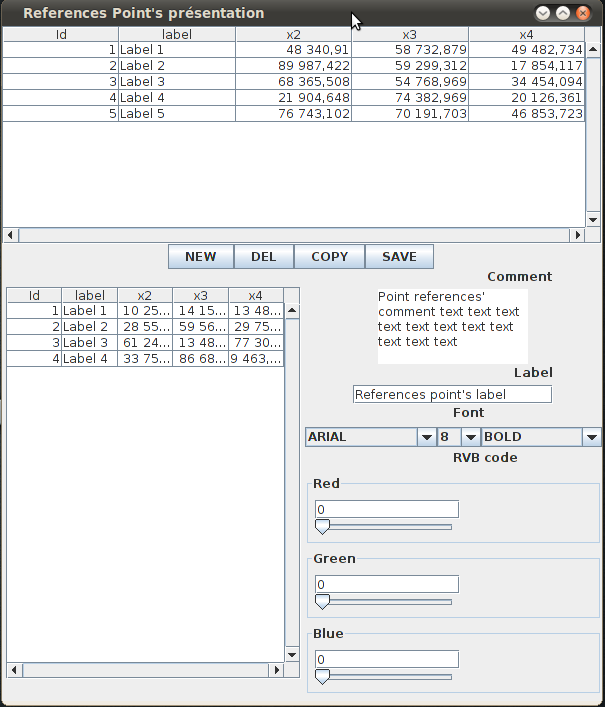
\includegraphics[scale=0.40]{spec-images/Onglet_PT.png}
  \caption{Onglet d'édition des Points de références}
\end{figure}

\paragraph{Utilisation de l'onglet :}

\begin{itemize}
\item Dans la partie supérieure, la liste des points de référence avec leur ID, leur label et leurs coordonnées pour les variables visualisées. Cette liste pourra ne comporter que les points actuellement visualisées, ou l'intégralité des points définis (choix au moyen d'un radio-bouton$\triangle$). Elle pourra être réordonnée, de façon croissante ou décroissante, selon les ID, les labels, et les valeurs des variables visualisées. Si la liste excède la taille de la zone dédiée, une barre de défilement verticale apparaîtra. La sélection, par clic gauche de la souris, d'un point de la liste le met également en surbrillance dans la fenêtre de visualisation. Réciproquement, la sélection d'un point dans la zone de visualisation sélectionne automatiquement celui-ci dans cette liste.
\item Quatres boutons séparant la partie supérieure de la partie inférieure:
  \begin{itemize}
  \item[.] New : Pour créer un nouveau point de référence. Il aura tous ces champs rempli de valeurs par défaut (paramétrables dans le menu Préférences).
  \item[.] Del : Pour supprimer le point de référence sélectionné.
  \item[.] Copy : Pour créer un nouveau point de références avec les même valeurs que celui sélectionné.
  \item[.] Save : Pour sauvegarder les modifications apportées dans la partie inférieure au point actuellement sélectionné.
  \end{itemize}
\item Dans la partie inférieure gauche, les coordonnées complétes (éditables) du point sélectionné dans la zone supérieure : la liste des valeurs de toutes les variables, munie au besoin d'une barre de défilement verticale, ordonnable (croissant ou décroissant) selon les noms des variables ou leurs valeurs.
\item Dans la partie inférieure droite, le label (éditable), un commentaire (éditable) et les caractéristiques d'affichage du point actuellement sélectionné :
  \begin{itemize}
  \item[.] La police utilisée pour le label
    \begin{itemize}
    \item[] Le nom de la police
    \item[] La taille de la police
    \item[] La mise en forme (gras, souligné, italique)
    \end{itemize}
  \item[.] 3 glissières associées à des champs textes permettant de personnaliser la couleur selon le codage RVB.
  \item[.] 1 glissière associée à un champ texte permettant de régler la taille du point de 1 à 10 pixels de diamètre. $\triangle$
  \end{itemize}
\end{itemize}

%----------------------------------------------------------------------------------
\subsection{Onglet Filters}\label{sec:onglet:flt}
\paragraph{Définition :} Un filtre (cf. partie \ref{sec:entree:entete}) permet de définir une règle que doivent valider les boites qui seront affichées. L'ensemble des filtres sont considérés en disjonction, c'est à dire que toute boite validant la règle d'au moins un filtre est affichée. La règle d'un filtre est une conjonction de conditions. Une condition porte sur n'importe quel élément d'une boite : son ID, les valeurs de ses variables, ses caractéristiques ; elle peut également être formulée comme une expression mathématique sur les variables de la boite (évaluée par arithmétique d'intervalles). La condition prend la forme d'une comparaison entre l'élément choisi et une valeur de référence. Les relations de comparaisons possibles et le type de la valeur de référence dépendent de l'élément choisi (cf. partie \ref{sec:entree:entete}).\\Les filtres sont gérés (créés, modifiés, supprimés) exclusivement depuis l'onglet Filters. Ils reçoivent un identifiant (IDInt) unique à leur création et celui-ci n'est pas modifiable, à l'inverse de toutes leurs autres caractéristiques.

\begin{figure}[!h] %on ouvre l'environnement figure
  \center
  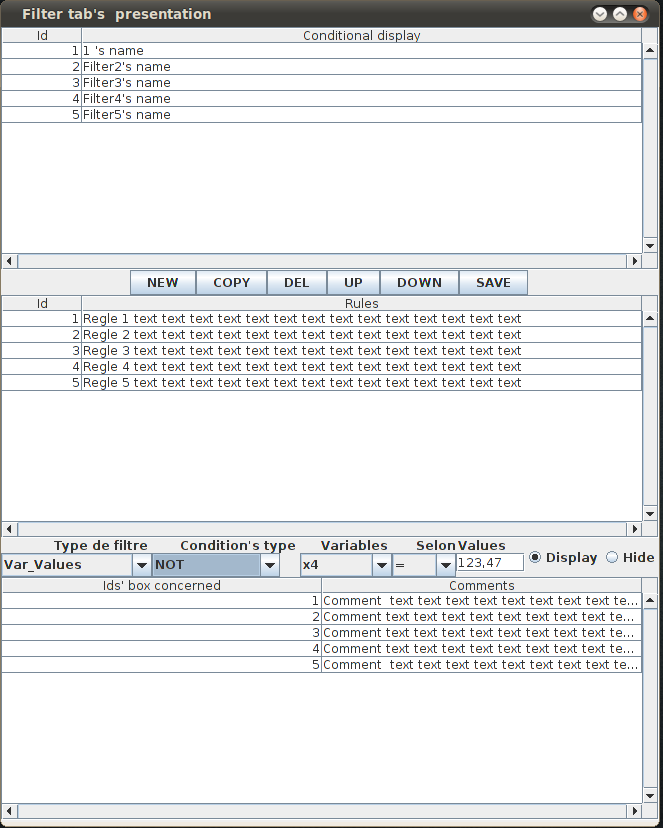
\includegraphics[scale=0.40]{spec-images/FilterTab.png} %ou image.png, .jpeg etc.
  \caption{Onglet de gestion des filtres} %la légende
\end{figure} %on ferme l'environnement figure

\paragraph{Utilisation de l'onglet :}

\begin{itemize}
\item Dans la partie supérieure, la liste des filtres avec leur ID, leur label (sous forme de champ texte directement éditable dans la liste), leur état $\triangle$ (actif ou inactif, sous forme de checkbox directement éditable dans la liste) et le nombre de boites qui valident leurs règles $\triangle$. Cette liste pourra être réordonnée, de façon croissante ou décroissante, selon les ID, les labels, l'état et le nombre de boites. Si la liste excède la taille de la zone dédiée, une barre de défilement verticale apparaîtra.
\item Quatres boutons séparant la partie supérieure de la partie inférieure:
  \begin{itemize} 
  \item[.] New : Pour créer un nouveau filtre vierge.
  \item[.] Del : Pour supprimer le filtre sélectionné.
  \item[.] Copy : Pour créer un nouveau filtre avec les même valeurs que celui sélectionné.
  \end{itemize}
\item Dans la partie inférieure, deux listes côte à côte :
  \begin{itemize}
  \item[.] la liste des conditions constituant la règle du filtre. Cette liste indique, pour chaque condition, l'élément testé, la relation de comparaison choisie, et la valeur de référence. La sélection d'une condition dans cette liste rempli les champs éditables se trouvant sous la liste avec les données correspondantes.
  \item[.] la liste des ID des boites validant la règle du filtre. La sélection d'une boite dans cette liste la sélectionne automatiquement dans l'onglet Box et la met en surbrillance dans la fenêtre de visualisation.
  \end{itemize}
  Sous la liste des conditions se trouvent des champs éditables permettant d'ajouter, modifier et supprimer une condition : $\triangle$
  \begin{itemize}
  \item[.] Un combobox pour le choix de l'élément testé (ID, variable, caractéristique, formule).
  \item[.] Une second combobox, permettant de choisir l'ID de la variable ou de la caractéristique concernée ; il est remplacé par un champ texte permettant de saisir la formule ; ou par rien du tout si l'élément testé est l'ID.
  \item[.] Un combobox permettant de choisir la relation.
  \item[.] Un champ texte permettant de saisir la valeur de référence ; le type de la donnée saisie sera validé selon la nature de l'élément testé (ID $\to$ entier positif ; variable, formule $\to$ Number ; caactéristique $\to$ Number ou String selon le type de la caractéristique).
  \item[.] un bouton "Add" pour ajouter une nouvelle condition (vierge).$\triangle$
  \item[.] un bouton "Mod" pour enregistrer les modifications apportées à la condition sélectionnée dans la liste au-dessus.$\triangle$
  \item[.] un bouton "Sup" pour supprimer la condition sélectionnée dans la liste au-dessus.$\triangle$
  \end{itemize}
\end{itemize}


%----------------------------------------------------------------------------------
\subsection{Onglet Conditional Style}\label{sec:onglet:aff}

\paragraph{Définition :} Un affichage conditionnel (cf. partie \ref{sec:entree:entete}) permet de définir un style d'affichage pour les boites vérifiant une certaine règle. L'ensemble des affichages conditionnels sont considérés en disjonction, mais dans l'ordre de leur priorité (entier positif de 1 à N s'il y a N affichages conditionnels définis), c'est à dire que toute boite utilisera le style du l'affichage conditionnel le plus prioritaire (plus petite valeur de priorité) dont elle satisfait la règle ; les boites ne satisfaisant aucune règle d'affichage conditionnel s'afficheront avec un style par défaut (paramétrable dans le menu Préférences). La règle d'un affichage conditionnel est identique à celle d'un filtre : c'est une conjonction de conditions portant sur n'importe quel élément d'une boite. Le style d'affichage des boites se résume à leur couleur et à leur degré de transparence, les deux étant définis simultanément selon le codage RVBA.\\Les affichages conditionnels sont gérés (créés, modifiés, supprimés) exclusivement depuis l'onglet Conditional Style. Ils reçoivent un identifiant (IDInt) unique à leur création et celui-ci n'est pas modifiable, à l'inverse de toutes leurs autres caractéristiques. La priorité par défaut d'un nouvel affichage conditionnel est d'être en dernière position; à la suppression d'un affichage conditionnel, les suivants gagnent une priorité (compactage).

\begin{figure}[!h] %on ouvre l'environnement figure
  \center
  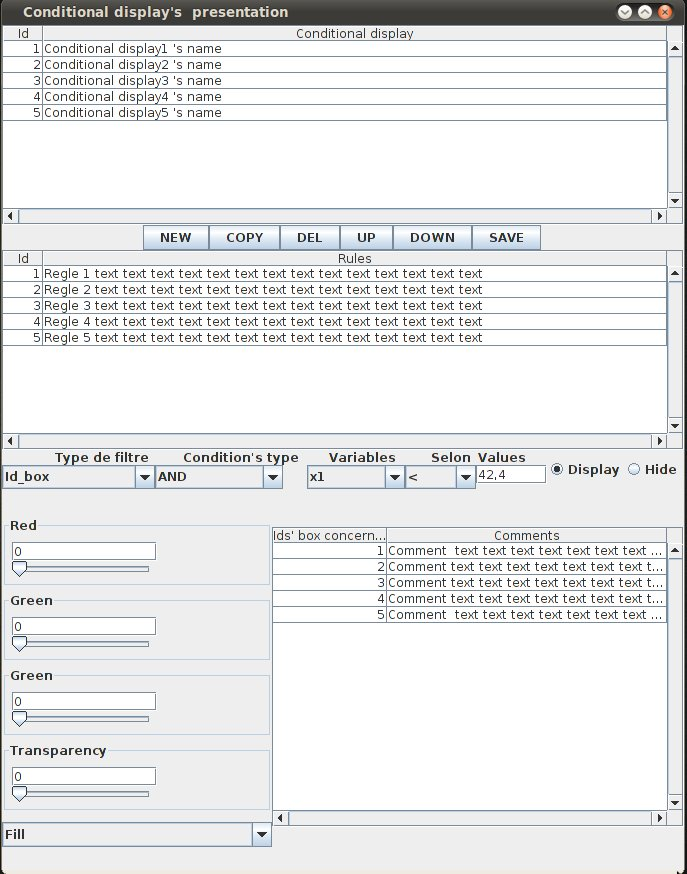
\includegraphics[scale=0.40]{spec-images/Aff_cond.jpeg} %ou image.png, .jpeg etc.
  \caption{Onglet de gestion des affichages conditionnels} %la légende
\end{figure} %on ferme l'environnement figure

\paragraph{Utilisation de l'onglet :}
\begin{itemize}
\item Dans la partie supérieure, la liste des affichages conditionnels avec leur ID, leur label (sous forme de champ texte directement éditable dans la liste), leur priorité $\triangle$ et le nombre de boites qui valident leurs règles $\triangle$. Cette liste pourra être réordonnée, de façon croissante ou décroissante, selon les ID, les labels, les priorités et le nombre de boites. Si la liste excède la taille de la zone dédiée, une barre de défilement verticale apparaîtra.
\item Cinq boutons séparant la partie supérieure de la partie inférieure:
  \begin{itemize}
  \item[.] New : Pour créer un nouvel affichage conditionnel vierge.
  \item[.] Del : Pour supprimer l'affichage conditionnel sélectionné.
  \item[.] Copy : Pour créer un nouvel affichage avec les même valeurs que celui sélectionné.
  \item[.] Up : augmente la priorité de l'affichage conditionnel sélectionné.
  \item[.] Down : diminue la priorité l'affichage conditionnel sélectionné.
  \end{itemize}
\item Dans la partie médiane, deux listes côte à côte :
  \begin{itemize}
  \item[.] la liste des conditions constituant la règle de l'affichage conditionnel sélectionné (cf. onglet Filters).
  \item[.] la liste des ID des boites validant la règle de l'affichage conditionnel sélectionné. La sélection d'une boite dans cette liste la sélectionne automatiquement dans l'onglet Box et la met en surbrillance dans la fenêtre de visualisation.
  \end{itemize}
  Sous la liste des conditions se trouvent des champs éditables permettant d'ajouter, modifier et supprimer une condition (cf. Onglet Filters).$\triangle$
\item Dans la partie inférieure, la définition du style de l'affichage conditionnel sélectionné : 4 glissières associées à des champs textes permettant de personnaliser la couleur et la transparence selon le codage RVBA.\\ SUPPRIMER LE COMBO ET LA NOTION DE COULEUR DE TRAIT.\\Un bouton Save permet d'enregistrer les modfications du style d'affichage.
\end{itemize}


%%%%%%%%%%%%%%%%%%%%%%%%%%%%%%%%%%%%%%%%%%%%%%%%%%%%%%%%%%%%%%%%%%%%%%%%%%%%%%%%%%%%%%%%%%%%%%%
\section{Sauvegarde-Exportation}

\paragraph{Définition :}
\begin{itemize}
\item
  Dans le cas d'une exportation textuelle, il s'agit simplement de la création d'un fichier de même nature que le fichier d'entrée avec en plus les données spécifiques à l'outil (cf  1.1) correspondantes au moment de la sauvegarde.
\item
  Une exportation en image sera aussi possible :
  \begin{itemize}
  \item
    Image bitmap (png, jpeg, ...)
  \item
    vectorielle (svg, eps, ...)
  \end{itemize}
\end{itemize}
\begin{figure}[h] %on ouvre l'environnement figure
  \center
  \bf \Huge Image absente
%  \includegraphics[scale=0.75]{spec-images/Enregistrer1.jpeg}
  \caption{Fenêtre d'enregistrement } %la légende
\end{figure} %on ferme l'environnement figure

\paragraph{Fonctionnement :}
Une boîte de dialogue de sauvegarde classique, accessible depuis le menu File, par la barre d'outil, ou par le raccourci Ctrl+S, permettra de choisir le dossier en parcourant une arborescence. Une combobox permettra de choisir parmi les différents formats cités dans la définition. Un autre permettra de choisir si l'export concerne la totalité su pavage, seulement le pavage filtré, ou seulement la portion apparaissant dans le panneau de visualisation.

%%%%%%%%%%%%%%%%%%%%%%%%%%%%%%%%%%%%%%%%%%%%%%%%%%%%%%%%%%%%%%%%%%%%%%%%%%%%%%%%%%%
\section{Visualisation }\label{sec:visualisation}
\begin{itemize}
\item Choix des une, deux ou trois variables à afficher. Cette sélection pourra s'opérer à l'aide de trois combobox présents dans la barre d'outils.
\item Sélection : une entité (boite ou point) est sélectionne par un clic du bouton gauche de la souris. L'objet sélectionné sera mis en surbrillance et sélectionne dans la liste de l'onglet correspondant.\\ ABANDONNER LA SELECTION MULTIPLE.
\item Zoom :
  \begin{itemize}
  \item[.] revenir à une vue globale homogène du pavage (filtré). Soit par une touche (\keystroke{F10}), soit par un bouton de la barre d'outil, soit par le menu menu «display» : «Zoom All».
  \item[.] zoomer/dézoomer (homogène) soit avec la molette de la souris dans la zone de visualisation (zoom centré sur la zone pointée sur la souris), soit par les touches \keystroke{+} et \keystroke{-} (clavier ou pavé numérique), soit par le menu «display» : «Zoom In/Out», soit en donnant directement le pourcentage de zoom (par rapport à la vue globale = 100\%) dans la barre d'outil, soit enfin par le menu contextuel.
  \item[.] zoom par dimension : idem zoom/dézoom homogène en maintenant la touche \keystroke{1}, \keystroke{2} ou \keystroke{3} (clavier ou pavé numérique) enfoncée.
  \end{itemize}
\item Déplacement :
  \begin{itemize}
  \item[.] Transposition 2D, soit avec les flèches du clavier, soit à la souris en maintenant le bouton gauche enfoncé.
  \item[.] Centrage sur le point de mire de la souris, soit grâce à la touche \keystroke{c} soit via le menu contextuel.
  \item[.] Définition textuel des range possible par le menu «display» : «ranges»
  \end{itemize}
\item Rotation (en visu 3D uniquement) : s'effectue en maintenant enfoncée la touche \Alt ou la molette de la souris et déplaçant la souris ou avec les flèches du clavier.
\end{itemize}

\end{document}
%%%%%%%%%%%%%%%%%%%%%%%%%%%%%%%%%%%%%%%%%%%%%%%%%%%%%%%%%%%%%%%%%%%%%%%%%%%%%%%%%%%
%%%%%%%%%%%%%%%%%%%%%%%%%%%%%%%%%%%%%%%%%%%%%%%%%%%%%%%%%%%%%%%%%%%%%%%%%%%%%%%%%%%
%%%%%%%%%%%%%%%%%%%%%%%%%%%%%%%%%%%%%%%%%%%%%%%%%%%%%%%%%%%%%%%%%%%%%%%%%%%%%%%%%%%
